\chapter{Creación de una pieza de arte sonoro generado con ayuda de GPT-4}
\label{chap:algorai}

% \defaultFontEpigraph{Imagination Is All You Need!\dots}{\cite{erkerImaginationAllYou2023}}
\defaultFontEpigraph{Imagination Is All You Need!\dots}{Erker, Schaffer, y Spanakis (2023)}


Como consecuencia de las pruebas y experimentos realizados con la API y el Playground de OpenAI para este trabajo, se generaron decenas de archivos con código cuyo resultado sonoro fue juzgado de cierto interés, independientemente de su adecuación a los requerimentos pasados por el prompt. Estos bloques de código están escritos tanto en SuperCollider como en Tidal Cycles. En el primer caso responden a peticiones muy concretas de texturas, timbres o sucesiones sonoras, en el Playground; en el segundo, a sesiones de \emph{livecoding} compartidas, asistidas por la API en \emph{AlgorAI}.

Ninguna de las construcciones de código conseguidas responden a un plan de una pieza completa, sino, más bien, a texturas sonoras continuas o con pocas variaciones en el tiempo. Por esta razón, el planteamiento de composición de una pieza a partir de estos materiales ha sido organizado absolutamente por el compositor-investigador. En este caso, se ha optado por organizar los sonidos elegidos en la DAW (\emph{Digital Audio Workstation}) \emph{Ardour}. Los procesados y efectos aplicados han sido mínimos, con el fin de mantener la esencia de los sonidos generados por GPT-4, limitándose a filtrados, cortes y compensación dinámica entre elementos. 

% La Figura \ref{fig:ardour} muestra la organización de los sonidos en la DAW.

% \begin{figure}
%     \captionqr{Captura de pantalla de la DAW Ardour con los sonidos generados por GPT-4 organizados por pistas en una composición de arte sonoro.}{https://vimeo.com/906122849?share=copy}{video}
%     \centering
%     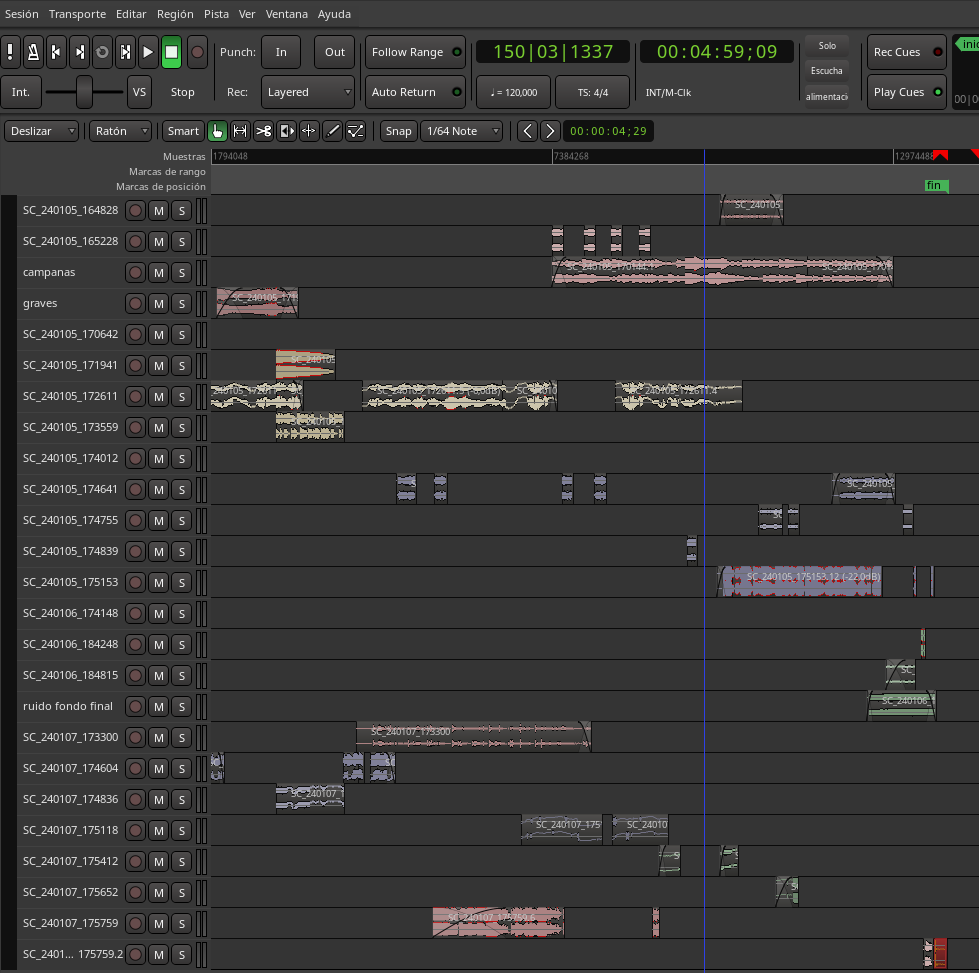
\includegraphics[width=0.8\textwidth]{./figuras/ardour.png}
%     \source{\propio}
%     \label{fig:ardour}
% \end{figure}


\section{Proceso y criterios de selección de material sonoro}

La selección de los fragmentos de código a utilizar en la composición se realizó en un momento distinto de la propia generación, hasta dos meses más tarde en algunos casos, sin atender a las intenciones primeras a la hora de dialogar con la API ni a su grado de adecuación a las peticiones. Se buscó, más bien, la variedad de texturas y timbres, así como la posibilidad de combinarlos entre sí en un discurso sonoro coherente y equilibrado. La búsqueda se realizó escuchando bloque por bloque y renderizando a archivos de audio una o varias versiones de los mismos, ya que en ocasiones el resultado sonoro dependía de factores externos al código como la posición o el movimiento del ratón en los ejes $X$ e $Y$. 

En el momento de la selección, se intentó encontrar una estructura base esquemática con la ayuda de GPT-4, pero siempre aparecían problemas asociados al entendimiento de los procesos en el tiempo por parte del LLM. Todas las soluciones eran extremadamente simples en el mejor de los casos, o bien lejos de lo que se pretendía, una composición temporal a partir de samples, en el peor y la mayoría de los casos. Por esta razón, se optó por la intervención humana absoluta en el proceso de composición, relegando el papel de GPT-4 a la generación de material sonoro.

\section{Descripción de la pieza}

\emph{AlgorAI}\footnote{La pieza puede ser escuchada en los enlaces de el códigos QR de la Figura \ref{fig:sonograma_algorai}} es una obra de música electroacústica. Su duración es de 5 minutos y está compuesta de un único movimiento, sin secciones claramente delimitadas. Su trama está compuesta por una sucesión polifónica de texturas sonoras de diversa índole, que se van superponiendo y combinando entre sí (véase una sección del sonograma de la Figura \ref{fig:sonograma_algorai}). Las decisiones de posición, duración y altura de cada sonido han sido tomadas en conjunto por el propio compositor, atendiendo a criterios subjetivos de equilibrio, coherencia e inteligibilidad desde el punto de vista psicoacústico. Su título, \emph{AlgorAI}, es un acrónimo de \emph{Algoritmo} e \emph{Inteligencia Artificial}, y hace referencia a la naturaleza de la obra, cuya materia prima sonora ha sido compuesta a partir de algoritmos de IA, en concreto, por grandes modelos de lenguaje. Los materiales sonoros son en su mayoría de origen íntegramente electrónico (aquellos producidos a través de SuperCollider), y en menor medida, de origen electroacústico (los producidos por Tidal Cycles), cuando la base de los mismos es un conjunto de \emph{samples} de sonidos reales.

\begin{figure}
    \captionqr{Sonograma de una parte de la pieza electroacústica \emph{AlgorAI}}{Sonograma de una parte de la pieza electroacústica \emph{AlgorAI}. Se puede apreciar parte de la trama polifónica creada por los diversos materiales sonoros que la componen.}{https://vimeo.com/906122849?share=copy}{video}
    \centering
    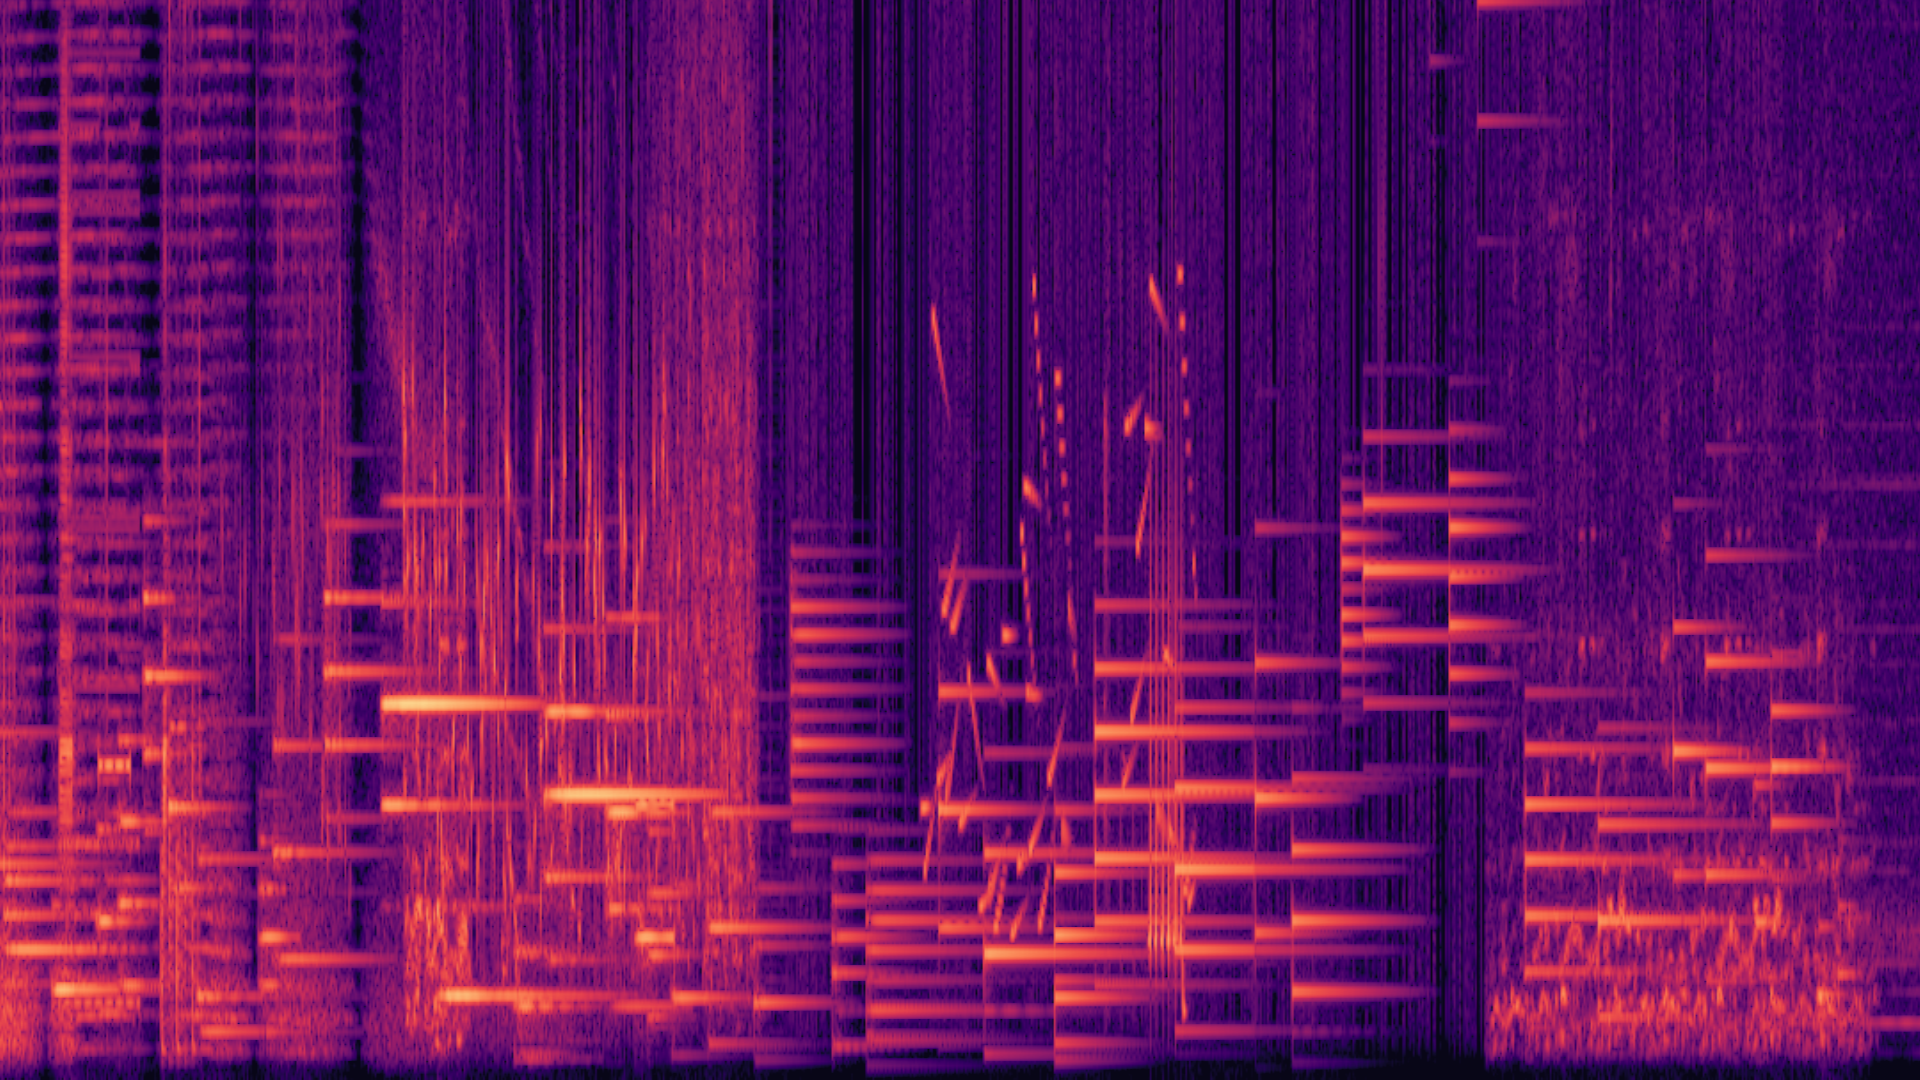
\includegraphics[width=0.8\textwidth]{./figuras/sonograma_02.png}
    \source{\propio}
    \label{fig:sonograma_algorai}
\end{figure}

\section{Técnicas de síntesis sonora utilizadas en los materiales sonoros}

Síntesis sustractiva, síntesis aditiva, frecuencia modulada, granulación y amplitud modulada son, en ese orden, las técnicas de síntesis sonora más utilizadas por GPT-4 en los experimentos en lo que la utilización del lenguaje de SuperCollider se refiere, independientemente de la petición en los prompts. La Figura \ref{fig:grafica_sintesis_gpt4} muestra esta distribución de uso de las técnicas de síntesis sonora utilizadas en los fragmentos de código que han servido como base de la composición. Se aprecia una tendencia a la síntesis sustractiva, aquella que consiste en filtrar armónicos de un sonido complejo, generalmente ruido blanco o clicks, para obtener sonidos complejos y ricos en matices.

\begin{figure}[H]
    \caption[Gráfica circular con la distribución de las técnicas de síntesis sonora utilizadas en los materiales sonoros generados por GPT-4 en SuperCollider]{Gráfica de barras con la distribución de las técnicas de síntesis sonora utilizadas en los materiales sonoros utilizados en la composición de \emph{AlgorAI}, generados por GPT-4 en SuperCollider. Se aprecia una clara tendencia a la utilización de la síntesis sustractiva.}
    \centering
    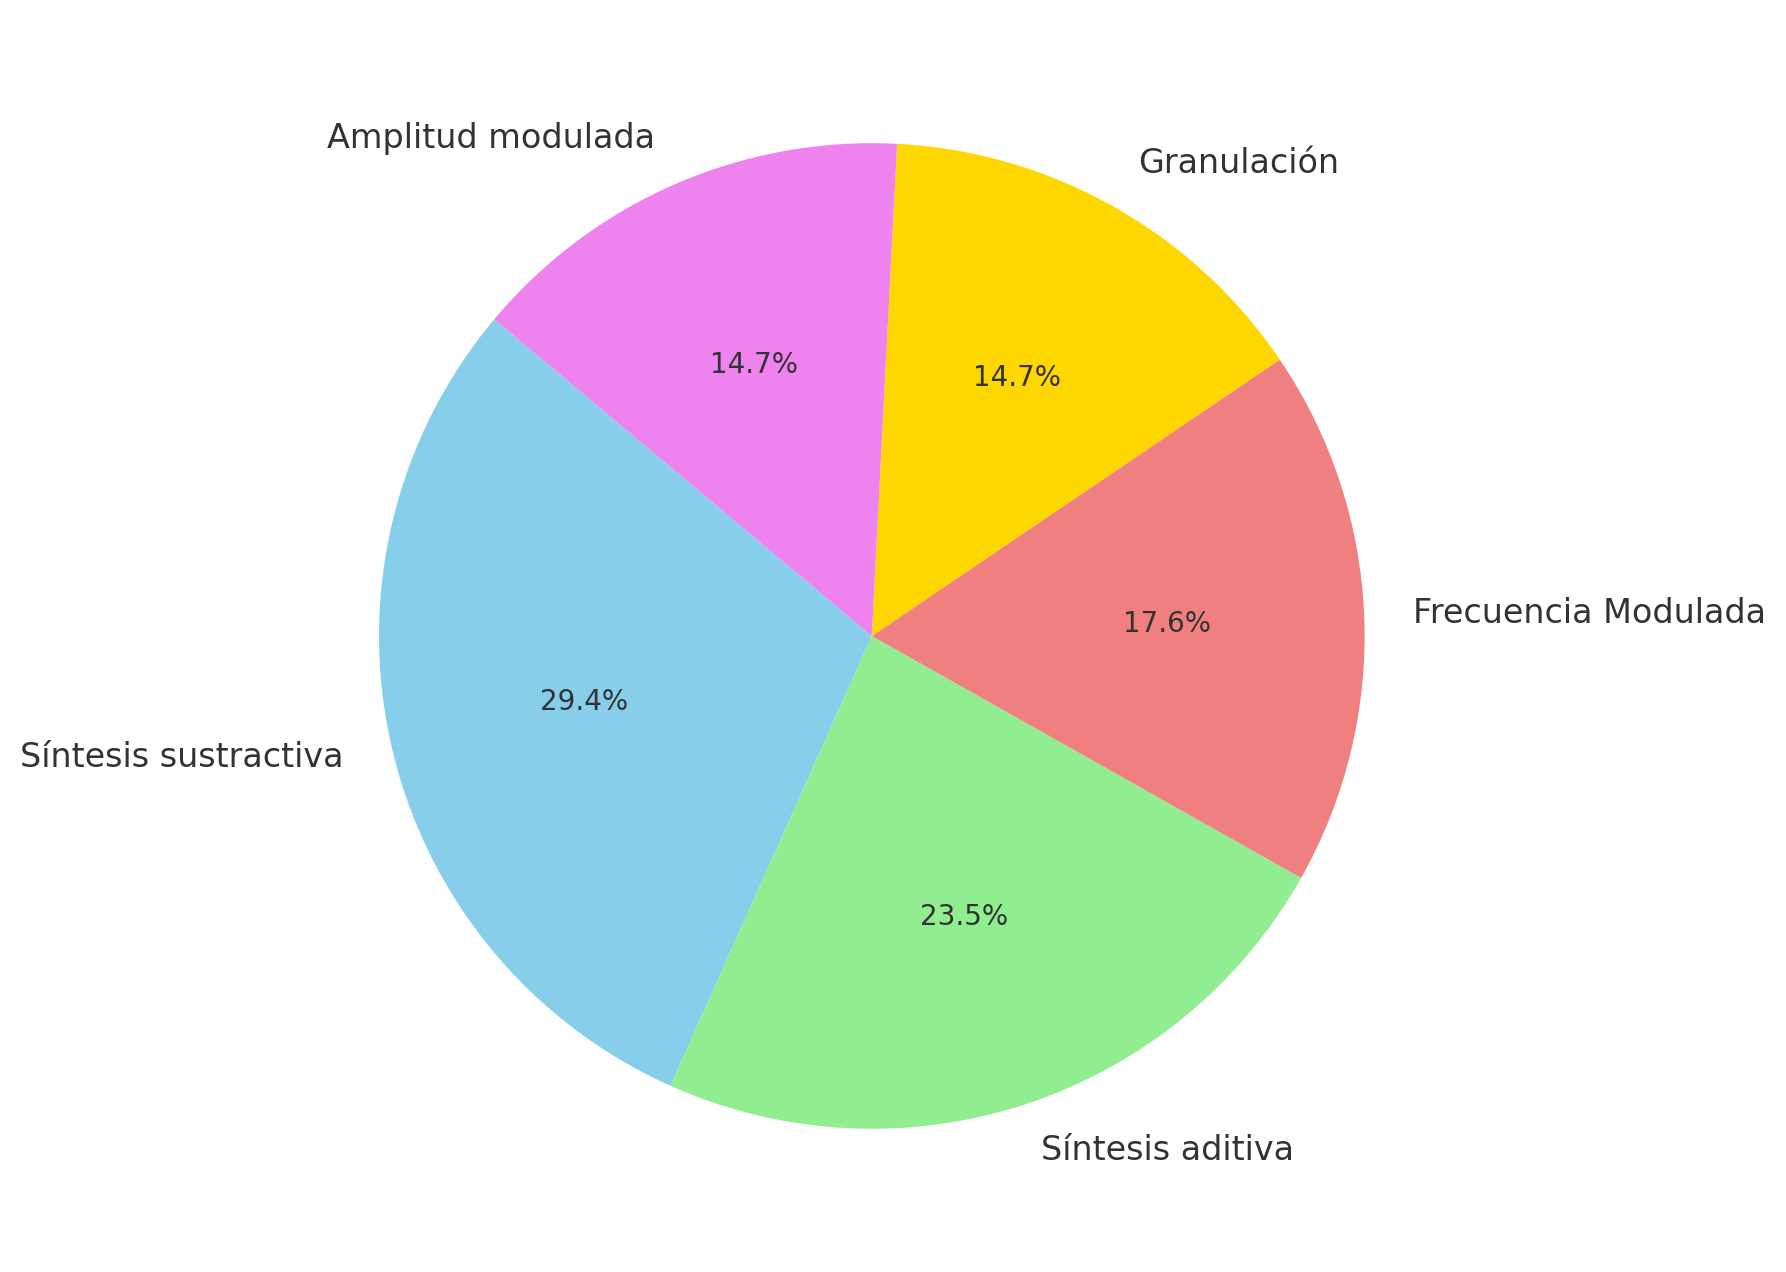
\includegraphics[width=0.8\textwidth]{./figuras/grafica_sintesis_gpt4_quesitos.png}
    \source{\propio}
    \label{fig:grafica_sintesis_gpt4}
\end{figure}

Una significativa parte de los materiales sonoros, a pesar de estar generados aparentemente por una técnica definida, en realidad deben su sonido más bien a combinaciones casuales y complejas, más fruto del azar que de la intención. Esto es común cuando los diversos parámetros de un sistema son llevados al extremo y producto sonoro es fruto de artefactos digitales como saturaciones, \emph{aliasing}, etc. Este aspecto de serendipia e impredecibilidad en la utilización de modelos de lenguaje aplicados a lo sonoro no es desdeñable, ya que puede ser una fuente de inspiración para el compositor.

Se aprecia una naturaleza distinta en los materiales generados en el lenguaje de Tidal Cycles, ya que este lenguaje se basa en la manipulación de samples y en su secuenciación en el tiempo. Los bucles más complejos que se aprecian en \emph{AlgorAI} han sido producidos por GPT-4 en Tidal Cycles. En este caso, se han escogido siempre los bucles sonoros más impredecibles, aquellos que no se ajustan a una estructura rítmica regular. La Figura \ref{fig:ejemplo_tidal_irregular} muestra uno de los ejemplos escritos en Tidal Cycles escogidos para la composición por su carácter irregular.


\begin{figure}[H]
    \captionqr{Ejemplo de código en Tidal Cycles escogido para la composición por su carácter irregular e impredecible}{Ejemplo de código en Tidal Cycles escogido para la composición por su carácter irregular e impredecible.}{https://drive.google.com/file/d/11KYkFOkBN42MlXUgHlmI8Rk2RWT7gQ8f/view?usp=drive_link}{audio}
    \centering
    \setstretch{1}
    \begin{lstlisting}[style=SuperCollider-IDE, basicstyle=\footnotesize\ttfamily, numbers=none]
d1 
    $ degradeBy 0.1
    $ slow 10 
    $ n (struct "[t(3,8)]*3 t(5,6) [t(6,7)]*4 t(3,4) t(2,3) t(7,8)"
        $ slow 3 
        $ ((fast 3 sine * rand) * (1-(fast 5 tri)) * (1-(fast 45 tri * rand))) *20) 
            # s "[[rash, cpu] | cpu2 | numbers | [arpy, <hi lo snare>] | [superpiano, [alphabet clap]?]]" 
            -- # s (choose["[rash, cpu]" , "[cpu2, hc]" ,"numbers" ," [arpy, <hi lo snare>]" , "[superpiano, [alphabet clap]?]"])
            # speed (slow 7 $ sine*1+0.05) 
            # legato 10
            # squiz (slow 20 $ sine*5)
            # room 1
            # size 0.8
            # delay 0.8
            # delaytime (choose [0.1, 0.5, 1])
            # delayfb 0.8
            # pan (range 0 1 rand)
            # vowel (slow 2.7 "{u o i e a i u a, a e i o u o}")
    \end{lstlisting}
    \source{\propio}
    \label{fig:ejemplo_tidal_irregular}
\end{figure}

\section{Interacción humano-LLM en el proceso de composición}

En este proceso compositivo, cabe preguntarse si la utilización de materiales sonoros generados por IA ha determinado en algún sentido la dirección y resultado final de la composición. En este caso, al menos en la apreciación subjetiva del compositor-investigador, la respuesta es negativa. La forma en la que se han combinado en el tiempo los diferentes materiales, su fraccionamiento, su duración, orden, etc., no estaba implícitos de ningún modo en los materiales sonoros, sino que responden a una decisión más o menos consciente y creativa del compositor. Otros materiales distintos hubieran dado lugar a otra pieza, aunque con un carácter y estilo similares. 

Sin embargo, no se puede considerar indiferente la utilización de materiales sonoros generados por IA en el proceso compositivo. En primer lugar, la utilización de estos materiales ha permitido al compositor-investigador explorar nuevas texturas y timbres que, de otro modo, no hubiera podido crear. El artista sonoro suele buscar sus materiales sonoros a modo de exploración, bien del mundo real, con micrófonos, bien del mundo electrónico o digital, experimentando con sintetizadores, secuenciadores y todo tipo de software de generación sonora. En este caso, la exploración realizada por medio de modelos de lenguaje en código de programación ha permitido al compositor-investigador dar con materiales que por sí mismo no hubiera podido crear, no por falta de conocimientos o habilidades, sino porque las posibilidades de combinación de elementos generadores es infinita, por una parte, y el creador humano tiende a repetir patrones y estructuras que le son familiares o que han resultado exitosas en el pasado, por otra.

En todo caso, es notable el ahorro de trabajo que ha supuesto el hecho de que el LLM haya generado los materiales sonoros. El tiempo necesario para ello se ha reducido con creces respecto a la creación de los mismos por parte del compositor. Podría objetarse que esto significa la pérdida del poder de control del artista sobre su obra, pero esto no es necesariamente cierto. La actitud del compositor humano frente al manejo del LLM por sus diferentes interfaces ha sido la de búsqueda y selección constante. Los archivos con código de los cuales se han elegido ciertos bloques para la composición puede que no lleguen a una tercera parte de todos los desechados en el proceso experimental. Los guardados como interesantes, a su vez, fueron el producto de varias iteraciones en el diálogo con el modelo. No se ha apreciado diferencia significativa en la calidad de la composición derivada de que el origen de los materiales sea la IA o producto de otras técnicas de exploración sonora. En todo caso, al tratarse de música experimental, la búsqueda de materiales ajenos a la intención del compositor es una constante, y la utilización de modelos de lenguaje en código de programación sonora se presenta como una herramienta más en el proceso de exploración sonora.

